\documentclass[a4paper, 14pt]{extarticle}

\usepackage{../latexDependencies/misc/preamble2}

\geometry{a4paper}

% Название дисциплины
\newcommand{\subject}{Теория автоматов и алгоритмические языки} 

% Тип работы
% lab - для лабораторной работы 
% hw  - для домашней     работы
\newcommand{\task}{hw} 

% Номер работы
\newcommand{\taskNumber}{2-1} 

% % Название работы
% \newcommand{\taskNameOne}{Определение списка полиномов интерполяционного} 
% \newcommand{\taskNameTwo}{сплайна третьей степени единичного дефекта} 
% \newcommand{\taskNameThree}{для заданной сеточной функции} 

% Имя студента
\newcommand{\studentName}{Очкин Н.В.}

% Имя преподававателя
\newcommand{\teacherName}{Кутыркин В.А.}

% Группа
\newcommand{\group}{ФН11-52Б}

% Вариант
\newcommand{\variant}{9}

\begin{document}

\graphicspath{ {../latexDependencies/images} } 
\normalsize

\newcommand{\printTask}{%
    \ifthenelse{\equal{\task}{lab}}{%
        лабораторной%
    }{%
        \ifthenelse{\equal{\task}{hw}}{%
            домашней%
        }{%
            Неизвестный тип задания%
        }%
    }%
}

\begin{titlepage}

    \begin{center}
        {\footnotesize \itshape Федеральное государственное бюджетное 
                       образовательное учреждение высшего образования}
    \end{center}

    \begin{minipage}[c]{0.1\textwidth}
        
\includegraphics[width=1.1\textwidth]{iconBMSTU}
    \end{minipage}
    \hfill
    \begin{minipage}[c]{0.9\textwidth}
        \centering
        \itshape
        \bfseries
        \small
        \guillemotleft Московский государственный технический университет \\
        имени Н.Э. Баумана\guillemotright \\
        (национальный исследовательский университет) \\
        (МГТУ им. Н.Э. Баумана) 
    \end{minipage}

    \vspace{0.5cm}
    \noindent\rule{\textwidth}{2pt} \\

    \noindent\uline{\textbf{ФАКУЛЬТЕТ} ФУНДАМЕНТАЛЬНЫЕ НАУКИ} \\
    \vspace{-5pt} \\
    \noindent\uline{\textbf{КАФЕДРА} ВЫЧИСЛИТЕЛЬНАЯ МАТЕМАТИКА И МАТЕМАТИЧЕСКАЯ} \\
    \vspace{-5pt} \\
    \noindent\uline{ФИЗИКА (ФН11)} \\
    \vspace{-5pt} \\
    \noindent\uline{\textbf{НАПРАВЛЕНИЕ ПОДГОТОВКИ} МАТЕМАТИКА И КОМПЬЮТЕРНЫЕ} \\
    \vspace{-5pt} \\
    \noindent\uline{НАУКИ (02.03.01)} \\

    \begin{center}
        \bfseries
        \textsc{О т ч е т} \\[10pt]
        по \printTask {} работе \textnumero {} \taskNumber
    \end{center}

    \vspace{10pt}

    \begin{center}
        \bfseries
        Вариант \textnumero {} \variant
    \end{center}

    \vspace{50pt}

    \hspace{10pt} 
    \noindent \textbf{Дисциплина:} \par
    \vspace{5pt}
    \hspace{10pt} 
    \noindent \subject

    \vspace{10pt}

    \begin{flushright}
        \renewcommand{\arraystretch}{3}
        \begin{tabular}{r r r}
            \multicolumn{1}{l}{Студент группы \uline{\group}} & 
            $\quad \underset{\text{(Подпись, дата)}}{\underline{\hspace{3cm}}} \quad$ & 
            \multicolumn{1}{c}{$\underset{\text{(И.О. Фамилия)}}{\uline{\textbf{\studentName}}}$} \\

            \multicolumn{1}{l}{Преподаватель} & 
            $\quad \underset{\text{(Подпись, дата)}}{\underline{\hspace{3cm}}} \quad$ & 
            \multicolumn{1}{c}{$\underset{\text{(И.О. Фамилия)}}{\uline{\textbf{\teacherName}}}$} \\
        \end{tabular}
    \end{flushright}

    \vfill

    \begin{center}
        \small
        Москва, 2024
    \end{center}
\end{titlepage}

\newgeometry{left=25mm, right=25mm, top=10mm, bottom=13mm}

\graphicspath{ {../latexDependencies/images/HW2-1} }

% Customize section, subsection, subsubsection and paragraph styles
\titleformat{\section}
  {\normalfont\large\bfseries}{\thesection}{1em}{}

\titleformat{\subsection}
  {\normalfont\normalsize\bfseries}{\thesubsection}{1em}{}

\titleformat{\subsubsection}
  {\normalfont\small\bfseries}{\thesubsubsection}{1em}{}

\titleformat{\paragraph}
  {\small\small\bfseries}{\theparagraph}{1em}{}

% \thispagestyle{empty}

% \null\newpage

% \setcounter{tocdepth}{5}
% \setcounter{secnumdepth}{5}

% \pagenumbering{roman}

% \tableofcontents
% \newpage

% \pagenumbering{arabic}
% \setcounter{page}{1}

\setstretch{1}
\linespread{1.1}

\setlength{\parindent}{0pt}

\fontsize{12pt}{16pt}\selectfont

% \definecolor{myblue}{HTML}{0A88C2}
% \definecolor{myred}{HTML}{FF1B1C}
% \definecolor{mygreen}{HTML}{386641}

% \lstdefinestyle{mystyle}{
%     basicstyle=\ttfamily\footnotesize,
%     keywordstyle=\color{myblue},
%     stringstyle=\color{myred},
%     commentstyle=\color{green!50!black},
%     showstringspaces=false,
%     frame=leftline, 
%     framesep=10pt, 
% }

% % Set the style for Python code
% \lstset{style=mystyle, extendedchars=\true}
% --------------------------------------START--------------------------------------

\section*{Задание}\vspace{-20pt}\rule{\linewidth}{0.1mm}

Для право-линейной грамматики создать автомат-анализатор. 
Продукции грамматики приведены ниже в таблице. Затем, инвертировав 
правые части продукций грамматики, получить лево-линейную грамматику 
и создать для неё автомат-анализатор. Сделать частичную проверку языка 
право- и лево-линейных грамматик, используя для этого автомат грамматики и 
автомат-анализатор языка автомата грамматики. Написать соответствующие 
правила вывода слов языка.

\section*{Исходные данные}\vspace{-20pt}\rule{\linewidth}{0.1mm}

\begin{center}
  \fontsize{17.28pt}{20.736pt}\selectfont 
  \bfseries
  Задача для право-линейной грамматики
  % $ \text{Таблица} \hspace{15pt} \to \hspace{15pt} \text{продукций} \hspace{15pt} \to \hspace{15pt} \text{грамматик} $
\end{center}

\vspace{-5pt}

\begin{figure}[h]
  \centering
  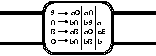
\includegraphics[page=1, scale=6]{graphics/data2}
\end{figure}

% \newpage

\vspace{-5pt}

\begin{center}
  \fontsize{17.28pt}{20.736pt}\selectfont 
  \bfseries
  Построим автомат право-линейной грамматики
\end{center}

% \vspace{-20pt}

\begin{figure}[h]
  \centering
  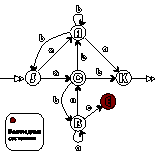
\includegraphics[page=1, scale=3.65]{graphics/diagramm1}
\end{figure}

\newpage
\newgeometry{left=25mm, right=25mm, top=20mm, bottom=20mm}

\begin{center}
  Произведем редукцию автомата относительно бесплодного состояния
\end{center}

\begin{figure}[h]
  \centering
  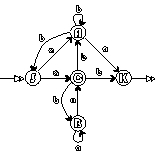
\includegraphics[page=1, scale=3.65]{graphics/diagramm2}
\end{figure}

Произведём детерминацию (синим цветом отмечены заключительные состояния)



\end{document}

% \begin{center}
%     \fontsize{12pt}{14.4pt}\selectfont 
%     \bfseries
%     \begin{tikzpicture}
%         % Draw the square
%         \draw (0,0) rectangle (5,5);
    
%         % Write the text inside the square
%         \node[align=left] at (2.5, 4) {S --> aC | aA\hphantom{ | cE}};
%         \node[align=left] at (2.5, 3) {A --> bA | bS | a\hphantom{C}};
%         \node[align=left] at (2.5, 2) {B --> aB | aC | cE};
%         \node[align=left] at (2.5, 1) {C --> bA | bB | b\hphantom{S}};

%         % Draw a bigger square
%         \draw (-0.1,-0.1) rectangle (5.1,5.1);
%     \end{tikzpicture}
% \end{center}